\section{Transformer \& Conformer in ASR}

\begin{frame}{}
    \LARGE \textbf{Transformer \& Conformer in ASR}
\end{frame}

\begin{frame}{Transformer \& Conformer in ASR}
    \begin{columns}
        \begin{column}{0.55\textwidth}
            \begin{itemize}
                \setlength{\itemsep}{1em}
                \item \textbf{Transformers} and \textbf{Conformers} are state-of-the-art architectures for Automatic Speech Recognition (ASR).
                \item Both leverage self-attention to model long-range dependencies in audio sequences.
                \item Conformer extends Transformer by integrating convolutional modules for local feature extraction.
                \item Key components include:
                    \begin{itemize}
                        \item Multi-head self-attention
                        \item Feed-forward networks
                        \item Residual connections and layer normalization
                    \end{itemize}
            \end{itemize}
        \end{column}
        \begin{column}{0.45\textwidth}
            \begin{figure}[h]
                \centering
                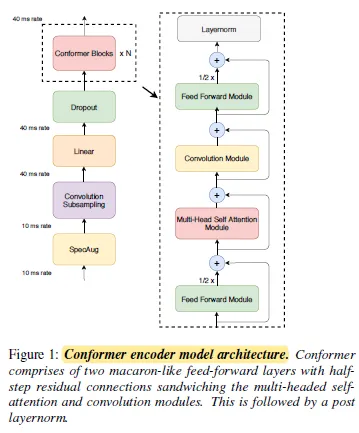
\includegraphics[width=\textwidth,height=0.9\textheight,keepaspectratio]{images/audio-nlp/transformer_conformer_overview.png}
            \end{figure}
        \end{column}
    \end{columns}
\end{frame}

\begin{frame}{Transformer Encoder: Core Components}
    \begin{itemize}
        \item \textbf{Multi-Head Self-Attention:}
        \begin{itemize}
            \item Captures global context by attending to all positions in the input sequence.
            \item Enables parallel processing of sequence data.
        \end{itemize}
        \item \textbf{Feed-Forward Network (FFN):}
        \begin{itemize}
            \item Applies non-linearity and projection to each position independently.
            \item Typical form:
            \begin{equation*}
                \mathrm{FFN}(x) = \mathrm{ReLU}(xW_1 + b_1)W_2 + b_2
            \end{equation*}
        \end{itemize}
        \item \textbf{Residual Connections \& Layer Normalization:}
        \begin{itemize}
            \item Stabilize training and improve gradient flow.
        \end{itemize}
    \end{itemize}
\end{frame}

\begin{frame}{Conformer Block (Gulati et al., 2020)}
    \begin{itemize}
        \item \textbf{Conformer} combines self-attention and convolution for effective speech modeling.
        \item \textbf{Block Structure:}
        \begin{itemize}
            \item Feed-Forward $\rightarrow$ Multi-Head Self-Attention $+$ Convolution $\rightarrow$ Feed-Forward
        \end{itemize}
        \item \textbf{Key Features:}
        \begin{itemize}
            \item \textbf{Convolution Module:}
            \begin{itemize}
                \item Gated Linear Units (GLU)
                \item Depthwise convolution for efficient local feature extraction
                \item Batch normalization for stable training
            \end{itemize}
            \item Residual connections and layer normalization throughout
        \end{itemize}
    \end{itemize}
\end{frame}




% \begin{frame}[allowframebreaks]{Transformer for ASR}

% \begin{itemize}
%     \item \textbf{Transformers} have revolutionized Automatic Speech Recognition (ASR).
%     \item Enable models to capture long-range dependencies in audio sequences using self-attention mechanisms.
%     \item Unlike traditional RNNs or CNNs, Transformers process entire sequences in parallel.
%     \item This parallelism leads to faster training and improved performance.
% \end{itemize}

% \begin{figure}[h]
%     \centering
%     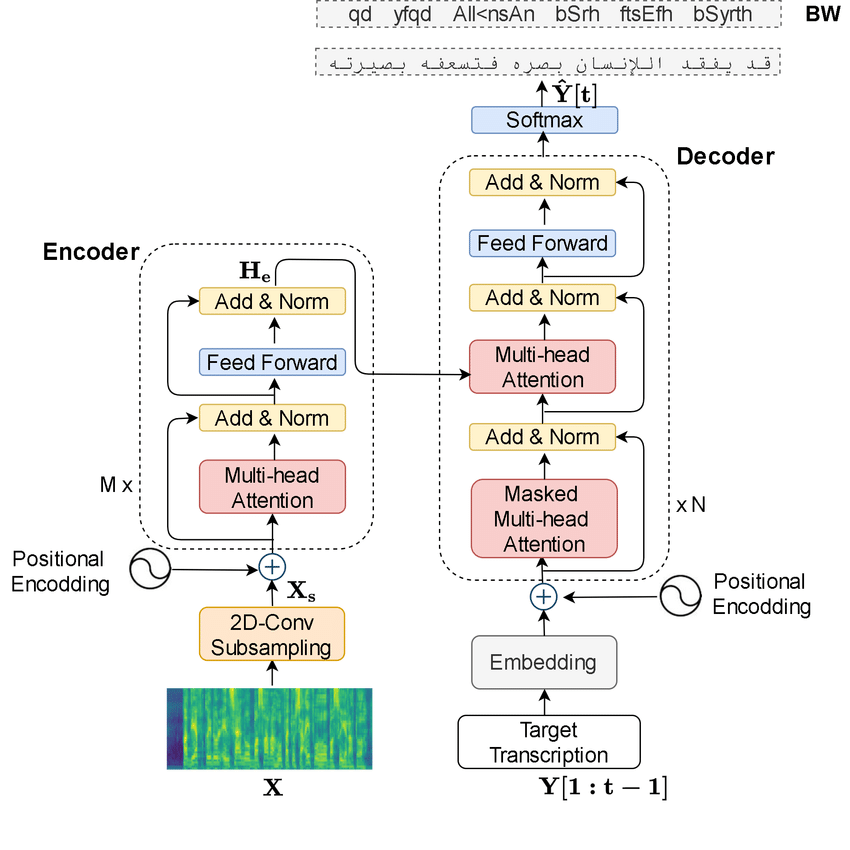
\includegraphics[width=\textwidth,height=0.8\textheight,keepaspectratio]{images/audio-nlp/transformer_architecture.png}
%     \caption*{Transformer architecture applied to ASR.}
% \end{figure}

% \textbf{Self-Attention Mechanism:}

% The core of the Transformer is the self-attention mechanism, which computes a weighted representation of the input sequence. The self-attention operation is defined as:

% \begin{equation}
% \mathrm{Attention}(Q, K, V) = \mathrm{softmax}\left(\frac{QK^T}{\sqrt{d_k}}\right)V
% \end{equation}

% where:
% \begin{itemize}
%     \item $Q$ (Query), $K$ (Key), and $V$ (Value) are projections of the input sequence.
%     \item $d_k$ is the dimension of the key vectors.
% \end{itemize}

% \begin{figure}[h]
%     \centering
%     \includegraphics[width=\textwidth,height=0.8\textheight,keepaspectratio]{images/audio-nlp/self_attention.png}
%     \caption{Self-attention mechanism in the Transformer.}
% \end{figure}

% \textbf{Position Encoding:}

% Since Transformers lack recurrence, they use position encodings to inject information about the order of the sequence. The most common approach is to use sinusoidal functions:

% \begin{equation}
% \begin{aligned}
% PE_{(pos, 2i)} &= \sin\left(\frac{pos}{10000^{2i/d_{model}}}\right) \\
% PE_{(pos, 2i+1)} &= \cos\left(\frac{pos}{10000^{2i/d_{model}}}\right)
% \end{aligned}
% \end{equation}

% where $pos$ is the position and $i$ is the dimension.

% \begin{figure}[h]
%     \centering
%     \includegraphics[width=\textwidth,height=0.8\textheight,keepaspectratio]{images/audio-nlp/positional_encoding.png}
%     \caption{Visualization of sinusoidal positional encoding.}
% \end{figure}

% \textbf{Summary:}

% \begin{itemize}
%     \item Transformers enable parallel processing and capture global context in ASR.
%     \item Self-attention allows the model to focus on relevant parts of the input sequence.
%     \item Position encoding provides sequence order information.
% \end{itemize}

% \end{frame}